\providecommand{\main}{..}
\documentclass[\main/main.tex]{subfiles}

\begin{document}
\section{Chapman-Kolmogorov equation}
\lesson{4}{08/10/20}
Let's see an application of the FP approach related to the \textit{first exit time} from a metastable state. The idea is to have a situation like the one in Figure \ref{fig:CK}, where we have two minima, $x_A, x_B$ and a barrier located at position $x_M$ that separates the two minima. We want to know - if my brownian particle is located in the metastable state around $x_A$ - how much time it takes on average to go over the energy barrier towards the stable state around $x_B$. We will call the exit time $\tau$.

\begin{figure}[h!]
   \centering
   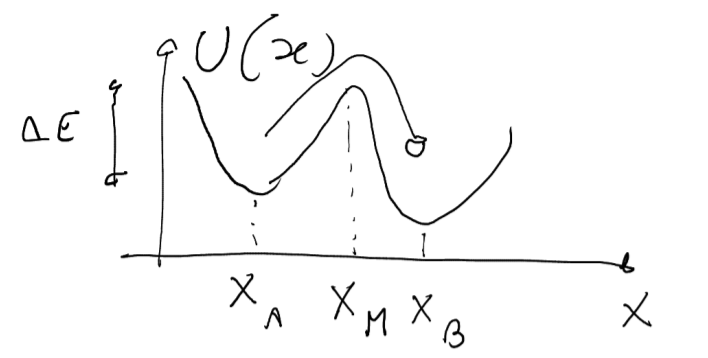
\includegraphics[width=0.7\linewidth]{Lectures/Images/well.png}
   \caption{Physical system with energy barrier $\Delta\epsilon$ and two minima used to calculate $\tau$.}
   \label{fig:CK}
\end{figure}

Arrhenius proposed a very simple formula: if we call $\Delta\epsilon$ the height of the energy barrier, according to Arrhenius $\tau\sim\exp(\frac{\Delta\epsilon}{k_B T})$. Using the FP formalism we will derive this formula and also a more precise formula, called \textit{Kramer's formula}, which include also the prefactors that are not present in the Arrhenius formula. \\

Let's start from the FP formalism in the contest of the \textit{Chapman-Kolmogorov} (CK) equation. Let's stress the fact that we are considering stochastic processes that are continuous in time, so we will write the continuous version of the CK equation in d=1.
The idea is to express the probability $W$ decomposing the steps going from time $t_0$ up to time $t+\Delta t$ in an interval that goes from $t_0$ to $t$ and then from $t$ to $t+\Delta t$. Since we are in a continuous time and in a continuous space we have to integrate on all possible spatial locations of the intermediate steps $y$:
\begin{eqnarray} 
W(x_0,t_0|x,t+\Delta t)= \int dy W(x_0,t_0|y,t) W(y,t|y,t+\Delta t)
\end{eqnarray}
Starting from this CK equation, one can derive a FP equation for $W$ that is known as \textbf{forward Kolmogorov equation} (FKE):
\begin{eqnarray}
\frac{\partial W(x_0,t_0|x,t)}{\partial t}=-\frac{\partial}{\partial x}(a(x,t) W(x_0,t_0|x,t))+ \frac{1}{2}\frac{\partial^2}{\partial x^2}(b(x,t)W(x_0,t_0|x,t))
\end{eqnarray}
where $W$ is a function of the starting position and of the starting time and of the arrival position/time. Forward means that we are considering FP with space and time derivatives with respect the arrival time and position. The expressions for $a$ and $b$ are similar to the ones described in the previous lectures. \\

One can derive this FKE but what we actually need is that we can use the same approach deriving a \textbf{Backward Kolmogorov equation} (BKE)\footnote{to see calculations appendix E: Kramer-Moyal expansion} with time and space derivatives with respect initial time and location:

\begin{eqnarray}
\frac{\partial W(x_0,t_0|x,t)}{\partial t_0}=-a(x_0,t_0)\frac{\partial}{\partial x_0}[ W(x_0,t_0|x,t)]-\frac{1}{2}b(x_0,t_0)\frac{\partial^2}{\partial x_0^2}[W(x_0,t_0|x,t)]
\end{eqnarray}

The BKE will be our starting point in order to calculate our\textit{ \textbf{first} average exit time}.
Let us define formally this problem: in general we are interested in the \textit{escape time} (or \textit{first exit time}) problem from an interval with $x_1$ and $x_2$ boundaries, $I=[x_1,x_2]$ (we are in 1d).
Our brownian particle is initially located in that in
interval and we want to compute how much time it takes to the particle in order to escape from this interval.
One key point in this computation is that we need at least one \textit{absorbing boundary}, for instance $x_2$, such that the probability of finding a particle at the boundary is zero for all times: $x_2\to p(x_2,t)=0$. 

Physically, if we think of probability as related to a concentration profile, saying that concentration at one boundary is zero means that once the particles reach that boundary they are immediatly taken away from the system.

We enphasize the fact that we are talking about \textit{first} exit time because the is \textbf{no reantrance} of the particles from outside of the system. It is also important to point out that the first exit time is a stochastic random variable. \\

The probability of remaining in the interval $I$ at time $t$ after having started in $x_0$ is defined as (using the conditional probability $W$):
\begin{eqnarray}
\mathbb{P}_{x_0}(t)=\int_{x_1} ^{x_2} W(x_0,t_0|y,t) dy
\label{eq:p_def}
\end{eqnarray}
In this way we are integrating over all possible locations of the particle at time $t$ within the interval and this gives me the probability of the particle of being in the interval at time $t$.
The point is having an absorbing boundary and with the condition of no rentrance of the particles in the system, this probability is similar to a cumulative distribution function (CDF), but why? \\
The first observation is that $\mathbb{P}_{x_0}(t)$ decreases with $t$ increasing; at the initial time $t_0$ the conditional probability is a Dirac delta, so:
\begin{eqnarray}
\mathbb{P}_{x_0}(t_0) = \int_{x_0} ^{x_1} \delta(y-x_0) dy = 1
\end{eqnarray}
and on the other hand, considering the limit of infinite time, we get that $\mathbb{P}_{x_0}(t)\overset{t \to\infty}{\longrightarrow}0$ because we have absorbing boundaries and no rentrance in the interval! \\
In other words we can say that $\mathbb{P}_{x_0}(t)$ is the probability that the exit time $\mathbb{T}_I(x_0)>t$. \\

Since $\mathbb{P}_{x_0}(t)$ is more similar to a CDF, we will call $\pi(t)$ its the corresponding PDF for the random variable $\mathbb{T}_I(x_0)$: we can obtain $\pi(t)$ as follows. To be precise the correct CDF is $1-\mathbb{P}$.
$$
\begin{cases}
\pi(t)=-\frac{d \mathbb{P}_{x_0}(t)}{dt} \\
\mathbb{P}_{x_0}=\int_t^{+\infty} \pi(\tau) d\tau
\end{cases}
$$
The quantity we are interested in is:
\begin{eqnarray}
\mean{\mathbb{T}_I}=\int_{t_0} ^{+\infty} \tau \pi(\tau)d\tau\overset{(a)}{=} t_0 + \int_{t_{0}} ^{+\infty} \mathbb{P}_{x_0}(\tau)d\tau
\end{eqnarray}
where in (a) we performed an integration BP and we used the assumption that $\lim_{t\to\infty} t\mathbb{P}_{x_{0}} = 0$. \\

Now the idea is to consider the BKE and to perform the integration (\ref{eq:p_def}) in order to change it into an equation for $\mathbb{P}$. In doing this we are simplifing the situation too the case of the presence of constant drift force (the $a$ term doesn't depend on time) and of homogeneus medium ($D$ doesn't depend on space and time).
\begin{eqnarray}
\frac{\partial W(x_0,t_0|y,t)}{\partial t}= a(x_0)\frac{\partial W(x_0,t_0|y,t)}{\partial x_0}+D\frac{\partial
^2}{\partial x_0 ^2 }[W(x_0,t_0|y,t)]
\end{eqnarray}

Here we changed the sign because $(\frac{\partial W}{\partial t_0}= - \frac{\partial W}{\partial t})$ due to the time translation invariance, which means that $W$ depends on $(t-t_0)$. \\

Now we integrate over $y$ from $x_1$ to $x_2$ and in this way we get an equation for our CDF:
\begin{eqnarray}
\frac{\partial\mathbb{P}_{x_0}(t)}{\partial t} = a(x_0)\frac{\partial}{\partial x_0} \mathbb{P}_{x_0}(t) + D \frac{\partial ^2}{\partial x_0 ^2}\mathbb{P}_{x_0}(t)
\end{eqnarray}
It is important to stress that we have used the BKE because we are interested in the dependence from the initial position of the particle.
To simplify the notation from now $x_0 \mapsto x$, where $x$ is the initial starting position, while we set $t_0=0$.

Integrating the previous equation over $t$ (with $\mathbb{P}_x(0)=1$ and $\mathbb{P}_x(+\infty)=0$) we get an equation for $\mean{\mathbb{T}_I (x)}$ as a function of the initial position $x$:
\begin{eqnarray}
a(x)=\frac{\partial}{\partial x} \mean{\mathbb{T}_I(x)}+D\derparstwo{x}\mean{\mathbb{T}_I (x)}=-1
\end{eqnarray}

Let's solve this equation. The general solution is: $\Phi(x):=\exp[\frac{1}{D}\int_{\Bar{x}} ^x a(y)dy]$, where $\Bar{x}\in I$ is any choice and doesn't really matter, the important thing is that the integration must stop at the initial position $x$ (which defines $\Phi$ as a function of $x$). 

\begin{eqnarray}
    \frac{d}{dx}[\Phi(x)\frac{d}{dx}\mean{\mathbb{T}_I}(x)]=-\frac{1}{D}\Phi(x)
\end{eqnarray}
If we substitute the expression of $\Phi$ in here we can notice that the two equations are equivalent. This expression can be solved with multiple integrations taking into account the appropriate boundary conditions:

\begin{eqnarray}
    \frac{d\mean{\mathbb{T}}_I (x)}{dx}=-\frac{1}{D}\frac{1}{\Phi(x)}\int_{x_1} ^x dy\Phi(y)
\end{eqnarray}
Here we are considering $x_1$ i.e. a \textit{reflecting boundary} which means that if $x=x_1 \implies \frac{d\mean{\mathbb{T}_I (x)}}{dx}|_{x=x_1}=0$: this is the first integration step.

The second integration step is the following: here we get an equation for the first exit time as a function of $x$

\begin{eqnarray}
    \mean{\mathbb{T}_I (x)}=-\frac{1}{D}\int_{x_2} ^x\frac{dy}{\Phi(y)}\int_{x_1}^y dz \Phi (z)
    \label{eq:miao}
\end{eqnarray}

The previous integration over $y$ becomes an integration over $z$. Here we are fixing the upper boundary condition: before we have used the BC at $x_1$, now we will fix the BC at $x_2$. In this way $\mean{\mathbb{T}_I (x_2)}=0$ because $x_2$ is an \textit{absorbing boundary} and it makes sense because if we start at $x_2$ the particle is already out and the exit time is zero. \\

What we had in mind since from the beginning was a situation like the one represented in Figure \ref{fig:CK} in order to compute the time it takes to the particle to go from the metastable state to the stable state: in the developed formalism we identify $x_2$ as the position of the stable state ($x_2=x_B$). On the other hand $x_1$ is a position somewhere in the steepest location where the potential energy is rising very quickly. The average exit time is not increasing moving $x_1$ further to the left in the limit of very high slope of the potential (reflecting BC). \\

The idea is that we are considering an initial position $x_0$ in the basin of the metastable state. The usual connection between the $a$ term with the drift velocity and external force is:
\begin{eqnarray}
    a(x)=v_0(x)=\frac{F(x)}{\Tilde{\gamma}}=-\frac{1}{\Tilde{\gamma}}\frac{d U}{dx}
\end{eqnarray}

Now we will rewrite the equation for $\Phi(x)$ using the previous definition of the $a$ coefficient:
\begin{eqnarray}
    \Phi(x)=\exp[-\frac{1}{D\Tilde{\gamma}}(U(x)-U(\Bar{x}))]
\end{eqnarray}

and finally the average exit time can be written in this way

\begin{eqnarray}
    \mean{\mathbb{T}(x)}=\frac{1}{D}\int_x ^{x_B}dy\exp(\frac{U(y)}{T})\int_{x_1}^y dz \exp(-\frac{U(z)}{T})
\end{eqnarray}

The '-' sign disappeared from (\ref{eq:miao}) because we inverted the boundaries of the first integral ($x_2$ is now on top and it is equal to $x_B$). On the other hand $U(\Bar{x})$ doesn't enter in the final expression for the average exit time and so far it is an exact equation and the only two assumptions that we made were about the BCs.

Now we will start doing an approximation: the relevant point is to understand how to approximate the $y$ dependence in the integral
\begin{eqnarray}
\exp(\frac{U(y)}{T})\int_{x_1}^y \exp(-\frac{U(z)}{T})dz
\label{eq:hh}
\end{eqnarray}

The point is that integrand is dominated by the first factor $\exp(\frac{U(x_M)}{T})$ for $y\sim x_M$ (i.e. when $y$ corresponds to the height of the barrier). The second factor doesn't contribue because, provided $\Delta\epsilon\overset{*}{>>}(U(x_A)-U(x_B))$, then in this case we are interested in the position where the potential energy is minimum (because we have $-U(z)$) and I am integrating from $x_1$ to $y$ and so when $y=x_M$ I already took into account the metastable state. Provided that the previous condition that we wrote is true and reminding that the stable state has less potential energy that the metastable state, the gain that I would have considering $y$ moving towards $x_B$ is not much because the energy difference between the stable and metastable states is much less than the height of the barrier. It is because of this assumption that we can say that the $y$ dependence is dominated by the first term of (\ref{eq:hh}). 

If we consider $y>x_M$ the gain that I have from the second term of (\ref{eq:hh}) is much less that the decrease that I have from the first factor. Physically this is the condition that makes the approximation (*) a sensible one.
\begin{eqnarray}
    \mean{\mathbb{T}_t(x)}\approx \frac{1}{D}\int_x^{x_B}dy\exp(\frac{U(y)}{T})\int_{x_{1}} ^{x_M} dz \exp(-\frac{U(z)}{T})
\end{eqnarray}
To sum up the crucial point was to approximate $y\approx x_M$ in the second integral: now we have two separate integrals and we can evaluate both of them as gaussian integrals, considering a Taylor expansion around the local maximum (which implies no first order) of the energy barrier of the potential energy, doing it for example for the first one
\begin{align}
    U(x)&=U(x_M)-\frac{1}{2}\alpha_2 (y-x_M)^2 \quad \textbf{where}\quad \alpha_2=-U{''}(x_M)>0\\
        &\approx \exp(\frac{U(x_M)}{T})\int_{x\to -\infty} ^{x_1 \to + \infty} dy \exp(-\frac{\alpha_2}{2 T}(y-x_M)^2) \\
        &\approx\sqrt{\frac{2\pi T}{\alpha_2}} \exp(\frac{U(x_M)}{T})
\end{align}
Then we can do similar approximation for the second integral (the only difference is that now we are expanding around the metastable state $x_A$ and $\alpha_1:=U''(x_A)>0$) and we get that $I_2\approx \sqrt{\frac{2\pi T}{\alpha_1}}\exp(-\frac{U(x_A)}{T})$.

Our final (approximate) result is:
\begin{eqnarray}
    \mean{\mathbb{T}_I(x)}\approx\frac{2\pi}{\sqrt{\alpha_1 \alpha_2}}\frac{T}{D}\exp(\frac{\Delta U}{T})
\end{eqnarray}
where $\Delta U=U(x_M)-U(x_A)$ and in this way we recovered the Arrhenius equation: as we can see if the diffusion coefficient is increasing the average exit time is decreasing (because particles can diffuse faster).




\end{document}